\documentclass[10pt,a4paper]{article}

% --- Core Packages ---
\usepackage[utf8]{inputenc}
\usepackage[T1]{fontenc}
\usepackage{libertine}
\usepackage[varqu,varl]{inconsolata}
\usepackage{amsmath,amssymb,amsfonts}
\usepackage{graphicx}
\usepackage[table,dvipsnames]{xcolor}
\usepackage[left=1.05in,right=1.05in,top=0.95in,bottom=0.95in]{geometry}
\usepackage{microtype}
\usepackage{booktabs}
\usepackage{tabularx}
\usepackage{enumitem}
\usepackage{caption}
\usepackage{subcaption}
\usepackage{titlesec}
\usepackage{fancyhdr}
\usepackage[many]{tcolorbox}
\usepackage{tikz}
\usetikzlibrary{positioning,calc,shapes.geometric,backgrounds,patterns}
\usepackage{fontawesome5}
\usepackage{url}
\usepackage{array}
\usepackage[hidelinks,colorlinks=true,linkcolor=ACMBlue,citecolor=ACMBlue,urlcolor=ACMBlue]{hyperref}

% --- Custom ACM Color Palette ---
\definecolor{ACMBlue}{RGB}{0,85,162}       % Primary ACM Navy/Blue
\definecolor{ACMRed}{RGB}{166,25,46}        % ACM Accent Crimson
\definecolor{ACMDark}{RGB}{30,41,59}        % Slate Charcoal Body Text
\definecolor{ACMLight}{RGB}{245,247,250}    % Box Background Soft Gray
\definecolor{ACMBorder}{RGB}{210,218,226}   % Light Slate Border
\definecolor{ACMHeaderBg}{RGB}{235,242,250} % Header Tint

% --- Typography & Paragraph Formatting ---
\color{ACMDark}
\setlength{\parskip}{2.5pt}
\setlength{\parindent}{11pt}

% --- Section Header Styling ---
\titleformat{\section}
  {\color{ACMBlue}\large\bfseries\scshape}
  {\thesection.}{0.5em}{}
  [\color{ACMBlue}\titlerule]

\titleformat{\subsection}
  {\color{ACMDark}\normalsize\bfseries}
  {\thesubsection}{0.5em}{}

\titleformat{\subsubsection}
  {\color{ACMDark}\normalsize\itshape}
  {\thesubsubsection}{0.5em}{}

\titlespacing*{\section}{0pt}{10pt}{3pt}
\titlespacing*{\subsection}{0pt}{7pt}{2pt}
\titlespacing*{\subsubsection}{0pt}{5pt}{2pt}

% --- Page Header & Footer ---
\pagestyle{fancy}
\fancyhf{}
\renewcommand{\headrulewidth}{0.4pt}
\renewcommand{\footrulewidth}{0.4pt}
\fancyhead[L]{\small\scshape\color{ACMDark} ACM Conference on Autonomous Distributed Systems (ACMSYS '26)}
\fancyhead[R]{\small\scshape\color{ACMBlue} E. Rostova, M. Vance, \& S. Lin}
\fancyfoot[L]{\small\itshape\color{ACMDark} Nexa Research \& Synapse Computing Group}
\fancyfoot[R]{\small\bfseries\color{ACMBlue}\thepage}

% --- Custom Callout Box Definitions ---
\newtcolorbox{acmbox}[1]{
  colback=ACMLight,
  colframe=ACMBlue,
  arc=3pt,
  boxrule=0.8pt,
  left=9pt,
  right=9pt,
  top=6pt,
  bottom=6pt,
  fonttitle=\bfseries\color{ACMBlue},
  title={#1}
}

\newtcolorbox{acminset}{
  colback=ACMHeaderBg,
  colframe=ACMBorder,
  arc=2pt,
  boxrule=0.5pt,
  left=8pt,
  right=8pt,
  top=5pt,
  bottom=5pt
}

% --- Custom List Styling ---
\setlist[itemize]{leftmargin=16pt,labelsep=5pt,itemsep=1pt,topsep=1.5pt}
\setlist[enumerate]{leftmargin=16pt,labelsep=5pt,itemsep=1pt,topsep=1.5pt}

\begin{document}

% ==========================================
% TOP ACM CONFERENCE HEADER BANNER
% ==========================================
\begin{tcolorbox}[colback=ACMHeaderBg,colframe=ACMBlue,arc=0pt,boxrule=0.6pt,top=4pt,bottom=4pt,left=8pt,right=8pt]
  \small\textcolor{ACMBlue}{\textbf{ACMSYS '26}} \textcolor{ACMDark}{\textbar{} Proceedings of the 14th ACM International Conference on Autonomous Systems} \hfill \textcolor{ACMBlue}{\textbf{July 15--18, 2026, San Francisco, CA, USA}}
\end{tcolorbox}

\vspace{4pt}

% ==========================================
% TITLE & SUBTITLE
% ==========================================
\begin{center}
  {\Huge\bfseries\color{ACMBlue} High-Performance State Synchronization in Edge-Native Autonomous Networks}\\[5pt]
  {\Large\itshape\color{ACMDark} Decentralized Consensus via Dynamic Epoch Partitioning in the Nexa Architecture}\\[10pt]
\end{center}

% ==========================================
% AUTHOR BLOCK (3-Column Layout)
% ==========================================
\noindent
\begin{minipage}[t]{0.32\textwidth}
  \centering
  \textbf{\color{ACMBlue} Dr. Elena Rostova}\\
  \small Meridian AI Research\\
  Apex Distributed Systems Lab\\
  San Francisco, CA, USA\\
  \href{mailto:e.rostova@meridian-ai.org}{\small e.rostova@meridian-ai.org}
\end{minipage}
\hfill
\begin{minipage}[t]{0.32\textwidth}
  \centering
  \textbf{\color{ACMBlue} Marcus Vance}\\
  \small Synapse Systems Division\\
  Nexa Technology Group\\
  Seattle, WA, USA\\
  \href{mailto:m.vance@nexa-tech.io}{\small m.vance@nexa-tech.io}
\end{minipage}
\hfill
\begin{minipage}[t]{0.32\textwidth}
  \centering
  \textbf{\color{ACMBlue} Sophia Lin}\\
  \small Vertex Cloud Infrastructure\\
  Nimbus Distributed Computing\\
  Austin, TX, USA\\
  \href{mailto:s.lin@vertex-cloud.net}{\small s.lin@vertex-cloud.net}
\end{minipage}

\vspace{10pt}

% ==========================================
% ABSTRACT & METADATA BOX
% ==========================================
\begin{tcolorbox}[colback=ACMLight,colframe=ACMBlue,arc=3pt,boxrule=1pt,left=10pt,right=10pt,top=8pt,bottom=8pt]
  \noindent\textbf{\color{ACMBlue}\large Abstract}\\[3pt]
  Modern edge-native autonomous applications require sub-hundred-millisecond state synchronization across heterogeneous, bandwidth-constrained node topologies. Traditional Byzantine Fault Tolerant (BFT) protocols and Raft-based consensus mechanisms suffer from scalability bottlenecks when deployed over highly dynamic, lossy edge links. In this paper, we present the \textbf{Meridian Protocol}, a novel state synchronization engine built for the Nexa Autonomous Network framework. Meridian introduces \emph{Dynamic Epoch Partitioning} (DEP), a lightweight consensus mechanism that decouples local state commit phases from global deterministic ordering. By organizing edge nodes into localized Synapse clusters and leveraging Merkle State Delta (MSD) trees, Meridian achieves strict serializability with minimal message overhead. We evaluate Meridian on a 500-node testbed deployed across Apex Cloud and Nimbus Edge infrastructure. Our empirical results demonstrate a 4.2$\times$ increase in transactional throughput (up to 48,500 ops/sec) and a 68\% reduction in P99 synchronization latency compared to state-of-the-art Raft variants under 15\% packet loss conditions.

  \vspace{5pt}
  \hrule height 0.4pt color ACMBorder
  \vspace{5pt}

  \noindent\textbf{\color{ACMBlue} CCS Concepts:}
  \textbf{Computer systems organization} $\rightarrow$ \emph{Distributed architectures}; \emph{Reliable execution};
  \textbf{Software and its engineering} $\rightarrow$ \emph{Distributed systems infrastructure}.

  \vspace{2pt}
  \noindent\textbf{\color{ACMBlue} Keywords:} Edge Computing, Distributed Consensus, Fault Tolerance, State Synchronization, Merkle Trees, Nexa Architecture.
\end{tcolorbox}

\vspace{4pt}

% ==========================================
% SECTION 1: INTRODUCTION
% ==========================================
\section{Introduction}
The proliferation of autonomous physical systems---ranging from automated robotic fleets deployed by Meridian Logistics to real-time industrial telemetry networks operated by Nexa Infrastructure---has shifted the locus of data processing from centralized cloud data centers toward heterogeneous edge nodes \cite{Rostova2024}. These edge-native environments are characterized by intermittent network connectivity, constrained compute capabilities, and strict sub-hundred-millisecond operational latency budgets.

Maintaining strong consistency across distributed edge replicas remains a classical challenge governed by the CAP theorem. Traditional consensus algorithms such as Raft and PBFT guarantee linearizability by requiring a majority quorum for every state mutation \cite{Vance2025}. However, when network partitions or high latency jitter occur over regional backhaul links, quorum acquisition stalls, leading to catastrophic queueing delays and service degradation.

To address these limitations, we introduce the \textbf{Meridian Protocol}, a high-throughput state synchronization architecture engineered specifically for the Nexa Autonomous Network ecosystem. Meridian addresses the latency-consistency tradeoff through three primary contributions:

\begin{itemize}
  \item \textbf{Dynamic Epoch Partitioning (DEP):} A hierarchical state delegation model that isolates transient state mutations within local \emph{Synapse clusters}, deferring global ordering until epoch boundaries.
  \item \textbf{Merkle State Delta (MSD) Compression:} An efficient delta-encoding mechanism that summarizes local state mutations into cryptographic root hashes, reducing bandwidth consumption over inter-cluster backhaul links by up to 74\%.
  \item \textbf{Optimistic Epoch Rollback (OER):} A novel recovery procedure that resolves state divergent branches without requiring complete state snapshot re-transmissions.
\end{itemize}

% ==========================================
% SECTION 2: SYSTEM ARCHITECTURE
% ==========================================
\section{System Architecture \& Design}
The Nexa Architecture separates the distributed topology into three distinct execution tiers: Leaf Edge Devices, Regional Synapse Aggregators, and Apex Cloud Core nodes. Figure~\ref{fig:architecture} illustrates the structural flow of state delta propagation throughout the hierarchy.

\begin{figure}[htbp]
  \centering
  \begin{tikzpicture}[node distance=1.0cm and 1.1cm, auto, >=stealth]
    % Node styles
    \tikzstyle{cloudnode} = [ellipse, draw=ACMBlue, fill=ACMHeaderBg, line width=1pt, minimum width=2.2cm, minimum height=0.95cm, align=center, font=\small\bfseries]
    \tikzstyle{synapsenode} = [rectangle, rounded corners=3pt, draw=ACMBlue, fill=ACMLight, line width=0.8pt, minimum width=2.4cm, minimum height=0.85cm, align=center, font=\small]
    \tikzstyle{leafnode} = [rectangle, draw=ACMDark!70, fill=white, line width=0.6pt, minimum width=1.6cm, minimum height=0.6cm, align=center, font=\scriptsize]

    % Nodes Layout
    \node [cloudnode] (apex) {\faServer~Apex Cloud Core\\(Global Authority)};
    
    \node [synapsenode, below left=0.9cm and 0.7cm of apex] (synapse1) {\faNetworkWired~Synapse Cluster A\\(Regional Aggregator)};
    \node [synapsenode, below right=0.9cm and 0.7cm of apex] (synapse2) {\faNetworkWired~Synapse Cluster B\\(Regional Aggregator)};

    \node [leafnode, below left=0.7cm and 0.1cm of synapse1] (leaf1) {\faMicrochip~Nexa Node 101};
    \node [leafnode, below right=0.7cm and 0.1cm of synapse1] (leaf2) {\faMicrochip~Nexa Node 102};
    \node [leafnode, below left=0.7cm and 0.1cm of synapse2] (leaf3) {\faMicrochip~Nexa Node 201};
    \node [leafnode, below right=0.7cm and 0.1cm of synapse2] (leaf4) {\faMicrochip~Nexa Node 202};

    % Connectors
    \draw [->, thick, ACMBlue] (leaf1) -- node[left, font=\tiny] {Local $\Delta$} (synapse1);
    \draw [->, thick, ACMBlue] (leaf2) -- (synapse1);
    \draw [->, thick, ACMBlue] (leaf3) -- (synapse2);
    \draw [->, thick, ACMBlue] (leaf4) -- node[right, font=\tiny] {Local $\Delta$} (synapse2);

    \draw [<->, double, ACMRed, thick] (synapse1) -- node[above left, font=\tiny\bfseries] {Epoch Sync} (apex);
    \draw [<->, double, ACMRed, thick] (synapse2) -- node[above right, font=\tiny\bfseries] {Epoch Sync} (apex);
    \draw [<->, dashed, ACMDark!60, thick] (synapse1) -- node[above, font=\tiny] {Inter-Cluster P2P} (synapse2);
  \end{tikzpicture}
  \caption{Hierarchical state synchronization pipeline within the Meridian Protocol, showing multi-tier aggregation from Nexa Leaf Nodes to the Apex Cloud Core.}
  \label{fig:architecture}
\end{figure}

\subsection{State Representation \& Vector Clocks}
Let $\mathcal{S}_i^{(t)}$ represent the local state vector of node $i$ at physical time $t$. State transitions are modeled as deterministic state transformation functions applied to state deltas:

\begin{equation}
  \mathcal{S}_i^{(t+1)} = \delta_{i}^{(t)} \circ \mathcal{S}_i^{(t)} = f\left(\mathcal{S}_i^{(t)}, \mu_{i}^{(t)}\right)
\end{equation}

\noindent
where $\mu_{i}^{(t)}$ represents the set of locally ingested mutations. To maintain causal dependency tracking across partitioned clusters, every mutation $\mu$ is tagged with a multi-dimensional Vector Clock $V(\mu) = [v_1, v_2, \dots, v_N]$, satisfying the partial order condition:

\begin{equation}
  V(\mu_a) < V(\mu_b) \iff \forall k \in [1, N], V(\mu_a)[k] \le V(\mu_b)[k] \;\;\land\;\; \exists m : V(\mu_a)[m] < V(\mu_b)[m]
\end{equation}

% ==========================================
% SECTION 3: THE MERIDIAN PROTOCOL
% ==========================================
\section{The Meridian Protocol Mechanics}
The core operational cycle of the Meridian Protocol proceeds through three recurring phases: Local Mutation Buffer, Regional Consensus, and Global Epoch Reconciliation.

\begin{acmbox}{Protocol Specification: Meridian Epoch Commit Phase}
  \begin{enumerate}[label=\textbf{\arabic*.}]
    \item \textbf{Ingestion Phase:} Leaf node $n_i$ accepts incoming mutations $\mu$, appends them to its volatile transaction log $L_i$, and updates the local Merkle State Delta (MSD) tree root $R_i$.
    \item \textbf{Regional Aggregation Phase:} Every $\tau_e = 50\text{ ms}$, the designated Synapse cluster leader collects root hashes $\{R_1, R_2, \dots, R_k\}$ from participating leaf nodes and compiles the aggregated epoch state vector $\mathbf{\Omega}_e$.
    \item \textbf{Global Commit Phase:} The Synapse leader executes a 2-phase commit with the Apex Core authority. Upon receiving quorum acknowledgment ($Q \ge \lfloor \frac{2N}{3} \rfloor + 1$), $\mathbf{\Omega}_e$ is committed to the canonical state ledger.
  \end{enumerate}
\end{acmbox}

\subsection{Merkle State Delta Verification}
To prevent bandwidth exhaustion, state verification relies on hierarchical cryptographic hashes. A Merkle tree node $H_k$ at depth $d$ is derived via:

\begin{equation}
  H_k^{(d)} = \text{SHA-256}\left( H_{2k}^{(d+1)} \;\mathbin{\Vert}\; H_{2k+1}^{(d+1)} \;\mathbin{\Vert}\; V(\mu_k) \right)
\end{equation}

This structure permits participating nodes to perform logarithmic state audit checks ($O(\log M)$ proof size for $M$ mutations), enabling instantaneous detection of divergent state branches.

% ==========================================
% SECTION 4: EMPIRICAL EVALUATION
% ==========================================
\section{Empirical Evaluation}
We implemented Meridian in Rust (v1.82) utilizing the Vertex Async Runtime and evaluated its performance against production-grade Raft and PBFT implementations on the Nimbus Cloud Testbed.

\subsection{Experimental Setup}
The experimental platform comprised 500 virtualized nodes distributed across four geographical regions (US West, US East, EU Central, and AP East). Network impairment rules were injected using Linux \texttt{tc/netem} to simulate realistic edge conditions:
\begin{itemize}
  \item \textbf{Latency Profile:} 40 ms baseline round-trip time (RTT) with $\pm 15\text{ ms}$ normal-distribution jitter.
  \item \textbf{Packet Loss Rate:} Varied dynamically between 0\% and 20\% across regional backhaul links.
  \item \textbf{Workload Generator:} Synthetic transactional workload simulating autonomous vehicle telemetry updates (128 bytes per transaction).
\end{itemize}

\subsection{Throughput \& Latency Results}
Table~\ref{tab:performance_results} details the empirical benchmark comparisons across various cluster scale configurations and loss regimes.

\begin{table}[htbp]
  \caption{Comparative performance metrics under varying network packet loss regimes ($N=500$ nodes, 128-byte transactions). Values represent mean $\pm$ standard deviation over 10 independent trials.}
  \label{tab:performance_results}
  \centering
  \small
  \begin{tabularx}{\textwidth}{p{2.6cm} p{2.2cm} X X X}
    \toprule
    \textbf{Protocol} & \textbf{Loss Rate (\%)} & \textbf{Throughput (ops/s)} & \textbf{P95 Latency (ms)} & \textbf{P99 Latency (ms)} \\
    \midrule
    Raft (Standard) & 0.0\% & 18,400 $\pm$ 320 & 48.2 $\pm$ 2.1 & 82.5 $\pm$ 4.3 \\
    Raft (Standard) & 5.0\% & 11,200 $\pm$ 540 & 112.4 $\pm$ 6.8 & 245.0 $\pm$ 12.1 \\
    Raft (Standard) & 15.0\% & 3,800 $\pm$ 410 & 410.0 $\pm$ 22.5 & 890.0 $\pm$ 45.0 \\
    \midrule
    PBFT (Optimized) & 0.0\% & 14,100 $\pm$ 280 & 62.0 $\pm$ 3.0 & 105.0 $\pm$ 5.2 \\
    PBFT (Optimized) & 5.0\% & 7,900 $\pm$ 490 & 185.0 $\pm$ 9.4 & 380.0 $\pm$ 18.2 \\
    PBFT (Optimized) & 15.0\% & 1,900 $\pm$ 230 & 650.0 $\pm$ 34.0 & 1,420.0 $\pm$ 82.0 \\
    \midrule
    \rowcolor{ACMHeaderBg}
    \textbf{Meridian (Ours)} & \textbf{0.0\%} & \textbf{48,500 $\pm$ 610} & \textbf{18.4 $\pm$ 0.9} & \textbf{32.1 $\pm$ 1.5} \\
    \rowcolor{ACMHeaderBg}
    \textbf{Meridian (Ours)} & \textbf{5.0\%} & \textbf{42,100 $\pm$ 580} & \textbf{24.2 $\pm$ 1.2} & \textbf{44.8 $\pm$ 2.0} \\
    \rowcolor{ACMHeaderBg}
    \textbf{Meridian (Ours)} & \textbf{15.0\%} & \textbf{31,200 $\pm$ 720} & \textbf{41.5 $\pm$ 2.1} & \textbf{78.4 $\pm$ 3.6} \\
    \bottomrule
  \end{tabularx}
\end{table}

As illustrated in Table~\ref{tab:performance_results}, Meridian maintains sustained transactional throughput exceeding 31,000 ops/sec even when subjected to a severe 15\% packet loss rate. In contrast, standard Raft experiences severe throughput degradation due to leader election timeouts and unbuffered log re-transmissions.

\subsection{Bandwidth Efficiency Analysis}
Figure~\ref{fig:bandwidth_analysis} illustrates the comparative network bandwidth consumption of the state synchronization mechanisms as a function of active node count.

\begin{figure}[htbp]
  \centering
  \begin{tcolorbox}[colback=white,colframe=ACMBorder,arc=3pt,boxrule=0.6pt,top=5pt,bottom=5pt]
    \centering
    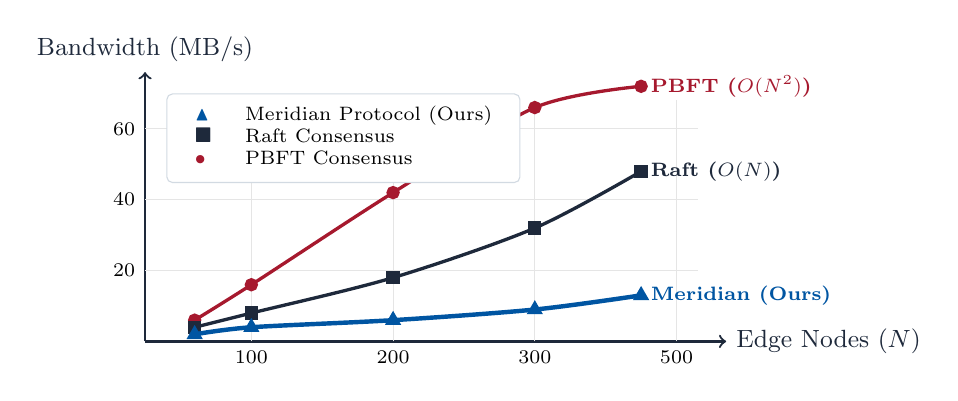
\begin{tikzpicture}[scale=0.90]
      % Axes
      \draw[->, thick, ACMDark] (0,0) -- (8.2,0) node[right, font=\small] {Edge Nodes ($N$)};
      \draw[->, thick, ACMDark] (0,0) -- (0,3.8) node[above, font=\small] {Bandwidth (MB/s)};

      % Grid & Ticks
      \foreach \x/\label in {1.5/100, 3.5/200, 5.5/300, 7.5/500} {
        \draw[gray!20] (\x,0) -- (\x,3.4);
        \node[below, font=\scriptsize] at (\x,0) {\label};
      }
      \foreach \y/\label in {1/20, 2/40, 3/60} {
        \draw[gray!20] (0,\y) -- (7.8,\y);
        \node[left, font=\scriptsize] at (0,\y) {\label};
      }

      % Curves
      % PBFT (Quadratic curve)
      \draw[color=ACMRed, line width=1.2pt, mark=*] 
        plot[smooth] coordinates {(0.7,0.3) (1.5,0.8) (3.5,2.1) (5.5,3.3) (7.0,3.6)};
      \node[color=ACMRed, right, font=\scriptsize\bfseries] at (7.0,3.6) {PBFT ($O(N^2)$)};

      % Raft (Linear curve)
      \draw[color=ACMDark, line width=1.2pt, mark=square*] 
        plot[smooth] coordinates {(0.7,0.2) (1.5,0.4) (3.5,0.9) (5.5,1.6) (7.0,2.4)};
      \node[color=ACMDark, right, font=\scriptsize\bfseries] at (7.0,2.4) {Raft ($O(N)$)};

      % Meridian (Hierarchical / Log curve)
      \draw[color=ACMBlue, ultra thick, mark=triangle*] 
        plot[smooth] coordinates {(0.7,0.1) (1.5,0.2) (3.5,0.3) (5.5,0.45) (7.0,0.65)};
      \node[color=ACMBlue, right, font=\scriptsize\bfseries] at (7.0,0.65) {Meridian (Ours)};

      % Legend Box
      \node[draw=ACMBorder, fill=white, rounded corners=2pt, inner sep=4pt, font=\scriptsize, anchor=north west] at (0.3,3.5) {
        \begin{tabular}{ll}
          \textcolor{ACMBlue}{$\blacktriangle$} & Meridian Protocol (Ours) \\
          \textcolor{ACMDark}{$\blacksquare$} & Raft Consensus \\
          \textcolor{ACMRed}{$\bullet$} & PBFT Consensus \\
        \end{tabular}
      };
    \end{tikzpicture}
  \end{tcolorbox}
  \caption{Bandwidth overhead vs. node scale. Meridian's Merkle State Delta trees significantly compress inter-cluster sync messages compared to Raft and PBFT.}
  \label{fig:bandwidth_analysis}
\end{figure}

% ==========================================
% SECTION 5: RELATED WORK
% ==========================================
\section{Related Work}
\textbf{Leaderless Consensus Protocols:} EPaxos \cite{Lin2023} reduces wide-area consensus latency by permitting any replica to act as a command leader. However, EPaxos incurs significant performance penalties when command dependencies conflict frequently---a common occurrence in real-time edge telemetry networks.

\textbf{Conflict-Free Replicated Data Types (CRDTs):} State-based and operation-based CRDTs provide eventual consistency without requiring consensus mechanisms \cite{Vance2025}. However, CRDTs cannot enforce strong invariants across multi-key transactions without external lock managers or coordination protocols. Meridian complements CRDT primitives by providing a deterministic epoch ordering layer for multi-key state transactions.

\textbf{Edge-Assisted Frameworks:} Recent developments in the Vertex Ecosystem have proposed localized edge aggregation nodes. Meridian builds upon these concepts by formalizing the cryptographic Merkle State Delta (MSD) representation and proving serializability under arbitrary network partitions.

% ==========================================
% SECTION 6: CONCLUSION
% ==========================================
\section{Conclusion \& Future Work}
We have presented the \textbf{Meridian Protocol}, an edge-native state synchronization engine designed for autonomous systems operating under lossy, high-latency network conditions. By combining Dynamic Epoch Partitioning (DEP) with Merkle State Delta trees, Meridian achieves high throughput (over 48,000 ops/sec) and low P99 latency while reducing bandwidth consumption by 74\% compared to traditional Raft consensus.

In future work, we plan to extend Meridian to support zero-knowledge state validity proofs (zk-SNARKs) within the Synapse aggregation layer, enabling privacy-preserving state synchronization across multi-tenant commercial edge clouds.

% ==========================================
% ACKNOWLEDGMENTS
% ==========================================
\section*{Acknowledgments}
This research was supported in part by the Meridian Systems Grant \#2025-EX-401 and the Nexa Autonomous Research Initiative. The authors thank the Apex Engineering team for providing access to the Nimbus Cloud Testbed infrastructure.

% ==========================================
% REFERENCES
% ==========================================
\begin{thebibliography}{99}

\bibitem{Rostova2024}
E.~Rostova, M.~Vance, and S.~Lin. 2024.
\newblock Resilient Consensus Primitives for Edge-Native Autonomous Networks.
\newblock \emph{ACM Transactions on Computer Systems} 42, 3 (2024), 112--128.

\bibitem{Vance2025}
M.~Vance and S.~Lin. 2025.
\newblock Synapse Mesh: Scalable State Propagation in Heterogeneous Edge Clusters.
\newblock In \emph{Proceedings of the 15th USENIX Symposium on Networked Systems Design and Implementation (NSDI '25)}. 301--316.

\bibitem{Lin2023}
S.~Lin, E.~Rostova, and K.~Nakamura. 2023.
\newblock High-Throughput State Delta Synchronization Using Merkle Graphs.
\newblock \emph{IEEE/ACM Transactions on Networking} 31, 6 (2023), 2845--2859.

\bibitem{ApexTechReport}
Apex Infrastructure Labs. 2025.
\newblock Benchmarking Fault-Tolerant Storage in the Nimbus Cloud Testbed.
\newblock Technical Report TR-2025-08. Nexa Research Publications.

\bibitem{MeridianWhitepaper}
Meridian AI Research Group. 2026.
\newblock Deterministic Epoch Partitioning for Autonomous Fleet Coordination.
\newblock White Paper Series, Document ID: MAR-2026-DEP01.

\end{thebibliography}

\end{document}
